\chapter{Setting up CA trees and HTTPS servers.}
\section{Introduction}
\paragraph{ }In this task, the \texttt{openssl toolkit} was used to set up a Certificate Authority and HTTPS servers in order to provide client/server authentication along with message confidentiality and integrity by passing the HTTP traffic over TLS. Note that although the CA has been set up in the \texttt{/root/ca} directory, the file structure has been copied over to the \texttt{tasks/Task 3} folder in the provided \texttt{.zip} file.

\section{Configuring the CA tree}
\paragraph{ }Initially, the terminal was set to run as root by running the command \texttt{sudo -i} and entering the password when prompted. The following commands were then run to create the directory structure as well as set restricted access to the directory. \\
\vspace{0pt}\\
\texttt{mkdir /root/ca\\
cd /root/ca\\
mkdir certs crl newcerts private\\
chmod 700 private\\
touch index.txt\\
echo 1000 > serial}

\paragraph{ }A configuration file was then set up, copying the contents from the \textit{Appendix} of the provided tutorial. this was saved in the file \texttt{/root/ca/openssl.cnf}. This file is important as it tells \texttt{openssl} what options to use when setting up the CA as well as the policies that must be followed by the CA intermediate signatures in order to get signed by the root CA. The root key was then created using \texttt{openssl} and this was encrypted using AES in order to be kept absolutely secure. The following code was run to do this, and a password was created when prompted.\\
\vspace{0pt}\\
\texttt{openssl genrsa -aes256 -out private/ca.key.pem 4096\\
chmod 400 private/ca.key.pem}

\paragraph{ }A root certificate was then set up using the newly created root key. The certificate was given an arbitrarily long expiry date of 7300 days for the sake of this assignment. After running the \texttt{openssl} command, details of the root CA were entered when asked to in order to be able to distinguish this CA from other CA's.
\begin{verbatim}
openssl req -config openssl.cnf \
    -key private/ca.key.pem \
    -new -x509 -days 7300 -sha256 -extensions v3\_ca \
    -out certs/ca.cert.pem
chmod 444 certs/ca.cert.pem
\end{verbatim}

\paragraph{ }The intermediate CA was then set up. In real world scenarios, the intermediate CA will be used to sign certificates on behalf of the root CA, so that the root CA can be kept  offline to improve the security of the structure. Thus, if the private key of the intermediate CA is compromised, the root CA will simply revoke the intermediate one. The following commands were run similar to those of creating the root CA in order to begin the setup of the intermediate CA. The last line in the following code adds a file to keep track of certificate revocation list, although this will not be used for this task, it was set up anyway to have a complete structure.
\begin{verbatim}
mkdir /root/ca/intermediate
cd /root/ca/intermediate
mkdir certs crl csr newcerts private
chmod 700 private
touch index.txt
echo 1000 > serial
exho 1000 > /root/ca/intermediate/crlnumber
\end{verbatim}

\paragraph{ }The intermediate CA configuration file was then set up similar to the root's configuration file, with a few commands changed. this was saved to \texttt{/root/ca/intermediate/ openssl.conf}. Once again, a key was then set up and the intermediate certificate was created and encrypted using the set up key. Note that the intermediate certificate was set to be valid for 3650 days, which is a shorter period than the root certificate.

\begin{verbatim}
cd /root/ca
openssl genrsa -aes256 \
    -out intermediate/private/intermediate.key.pem 4096

chmod 400 intermediate/private/intermediate.key.pem
openssl req -config intermediate/openssl.cnf -new -sha256 \
    -key intermediate/private/intermediate.key.pem \
    -out intermediate/csr/intermediate.csr.pem
    
openssl ca -config openssl.cnf -extensions v3_intermediate_ca \
    -days 3650 -notext -md sha256 \
    -in intermediate/csr/intermediate.csr.pem \
    -out intermediate/certs/intermediate.cert.pem
chmod 444 intermediate/certs/intermediate.cert.pem
\end{verbatim}

\paragraph{ }The \texttt{index.txt} file of the root CA was then checked to ensure that it contains an entry to the intermediate CA. After this, the certificate chain file was then created, this file tells the web browser how to complete the chain of trust when verifying a certificate in order to reach the root CA.

\begin{verbatim}
cat intermediate/certs/intermediate.cert.pem \
    certs/ca.cert.pem > intermediate/certs/ca-chain.cert.pem
chmod 444 intermediate/certs/ca-chain.cert.pem
\end{verbatim}

\section{Signing a domain using the CA}
\paragraph{ }In this task, the newly set up intermediate CA was used to sign a certificate for the domain \texttt{www.example.com}, thus enabling HTTPS access to the website. Firstly, a key was created for the client domain. Since this was set to expire after only 1 year, 2048 bits was used for the key instead of 4096 bits as this would be sufficiently secure and would increase the performance of TLS handshakes.

\begin{verbatim}
cd /root/ca
openssl genrsa -aes256 \
    -out intermediate/private/www.example.com.key.pem 2048
chmod 400 intermediate/private/www.example.com.key.pem
\end{verbatim}

\paragraph{ }Similar to the previous tasks, the private key was then used to create the certificate which will be signed by the intermediate CA using the following code, where the details of the domain were entered when prompted.

\begin{verbatim}
openssl req -config intermediate/openssl.cnf \
    -key intermediate/private/www.example.com.key.pem \
    -new -sha256 -out intermediate/csr/www.example.com.csr.pem

openssl ca -config intermediate/openssl.cnf \
    -extensions server_cert -days 375 -notext -md sha256 \
    -in interediate/csr/www.example.com.csr.pem \
    -out intermediate/certs/www.example.com.cert.pem
chmod 444 intermediate/certs/www.example.com.cert.pem
\end{verbatim}

\paragraph{ }After the above code was run, an entry was created in the \texttt{intermediate/index.txt} which referred to the new certificate of \texttt{www.example.com}. Once the CA tree was set up, with the domain certified, the \texttt{SSLCertificateFile} and \texttt{SSLCertificateKeyFile} entries in the Apache 2 settings file were changed to point to \texttt{/root/ca/intermediate/cert s/www.example.com.cert.pem} and \texttt{/root/ca/intermediate/private/www.example.com .key.pem} respectively. Finally, the following code was run to restart the server:

\begin{verbatim}
sudo a2enmod ssl
sudo service apache2 restart
\end{verbatim}

\paragraph{ }In order to verify that the server is working correctly, running \texttt{service apache2 status} gave the following output:

\begin{figure}[!h]
	\centering
	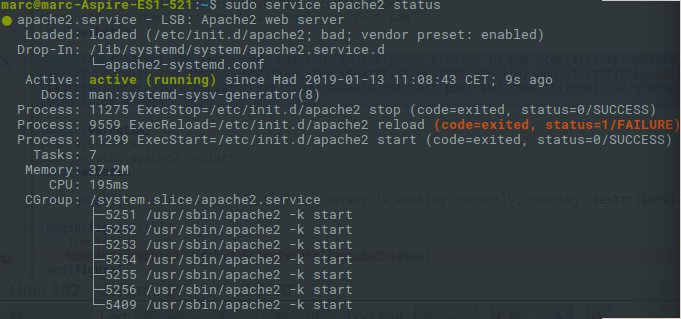
\includegraphics[width=0.6\textwidth]{apache2status}
\end{figure}

\paragraph{ }Furthermore, running \texttt{localhost} in a web browser or \texttt{https://localhost} both gave a running web page. Finally, the server's IP address was hard-coded in a DNS response cache file in order to carry out domain name resolution.

\section{Traffic Analysis on HTTP and HTTPS} 